\title{Lecture 4: Function and Graph}
\date{}
\frame{\titlepage}
\newcommand{\axes}[4]{\draw[<->](#1,0) -- (#2,0) node[right] {$x$}; \draw[<->](0,#3)--(0,#4) node[above] {$y$};}

%%%%%%%%%%%%%
\section{Function}
\frame{\sectionpage}
%%%%%%%%%%%%%

\begin{frame}
\begin{defn}{}{}
If a variable $y$ depends on a variable $x$ in such a way that each value of $x$ determines exactly one value of $y$, we say that $y$ is a function of $x$.
\end{defn}

Five common methods for representing functions are:
\begin{enumerate}
\item Numerically by tables
\item Abstractly by sets
\item Algebraically by formulas
\item Geometrically by graphs
\item Verbally
\end{enumerate}
\end{frame}

\begin{frame}
\frametitle{1. Numerically by tables}
\begin{table}[h!]
\centering
\begin{tabular}{|C||C|C|C|C|C|C|}
\hline
x & - 1.1&-1.01 & -1.001 & -0.999 & -0.99 & -0.9 \\
\hline
y & \pa 0.9 & \pa 0.99 & \pa 0.999 & \pa 1.001 & \pa 1.01 & \pa 1.1\\
\hline
\end{tabular}
\end{table}
\end{frame}


\begin{frame}
\frametitle{2. Abstractly by sets}
As a relationship from one set to another.
\begin{figure}[h!]
\centering
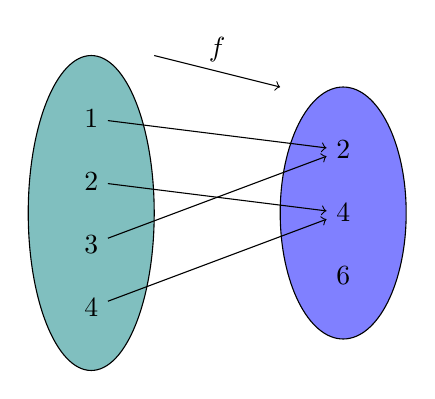
\begin{tikzpicture}[scale = 0.8]
\filldraw[fill = teal!50!white] (1,2.5) ellipse [x radius = 1, y radius = 2.5];
\filldraw[fill = blue!50!white] (5,2.5) ellipse [x radius = 1, y radius = 2];
\node at (1,4) (a1) {1};
\node at (1,3) (a2) {2};
\node at (1,2) (a3) {3};
\node at (1,1) (a4) {4};
\node at (5,3.5) (b1) {2};
\node at (5,2.5) (b2) {4};
\node at (5,1.5) (b3) {6};
\draw[->] (a1) -- (b1);
\draw[->] (a2) -- (b2);
\draw[->] (a3) -- (b1);
\draw[->] (a4) -- (b2);
\draw[->, bend angle = 45] (2,5) -- (4,4.5) node [pos = 0.5, above] {$f$};
\end{tikzpicture}
\caption{A function as a relationship between objects}
\end{figure}
\end{frame}

\begin{frame}
\frametitle{3. Algebraically by formulas}
As a machine that takes an input $x$ and gives a consistent output $y$.
\begin{figure}[h!]
\centering
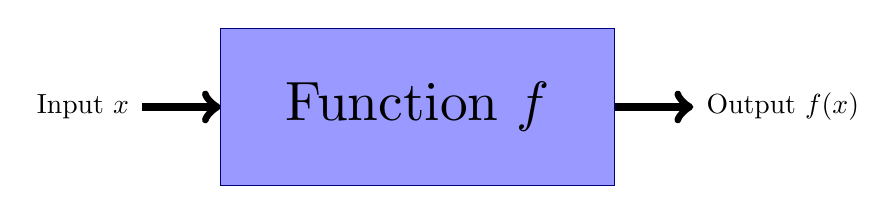
\begin{tikzpicture}
\draw[->, line width = 3] (-1,1) -- (0,1) node [left, pos=0] {Input $x$};
\filldraw[fill = blue!40!white, draw=blue!50!black] (0,0) rectangle (5,2);
\node at (2.5,1) [scale = 2] {Function $f$};
\draw[->, line width = 3] (5,1) -- (6,1) node [right] {Output $f(x)$};
\end{tikzpicture}
\caption{A function as a machine}
\end{figure}
\end{frame}

\begin{frame}
\frametitle{Fourth concept}
As points on a plane.
\addfig{0.8}{covid_graph}{COVID cases (October 10th)}{}
\end{frame}

\begin{frame}
\begin{figure}[h!]
\centering
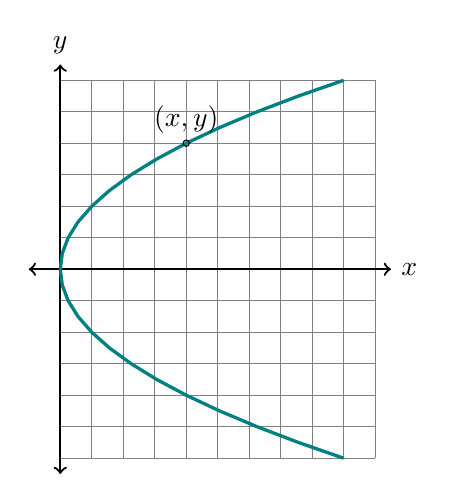
\begin{tikzpicture}[domain=-3:3, scale = 0.4]
\draw[help lines] (0,-6) grid (10,6);
\draw[<->, thick] (-1,0) -- (10.5,0) node[right] {$x$};
\draw[<->, thick] (0,-6.5) -- (0,6.5) node[above] {$y$};
\draw[color=teal, variable = \t, very thick] plot ({\t*\t},{\t*2});
\draw (4,4) circle [radius = 0.1cm] node[above] {$(x,y)$};
\end{tikzpicture}
\caption{A function as points $(x,y)$ on the plane.}
\end{figure}
\end{frame}

\begin{frame}
\frametitle{Fifth Concept}
Sometimes functions are described in words.
\begin{remark}{Newton's Law of Universal Gravitation}
The gravitational force of attraction between two bodies in the Universe is directly proportional to the product of their masses and inversely proportional to the square of the distance between them.
\end{remark}
This is the verbal description of the formula
\[F = G \frac{m_1 m_2}{r^2}\]
where $F$ is defined as a function of $r$.
\end{frame}


\begin{frame}
\frametitle{Formal definition}
\begin{defn}{}{}
A function needs to give only one output for any input.
\medskip

We write 
\[ f: A \rightarrow B\] 
to represent a function $f$ from the set $A$, called \textbf{Domain}, to the set $B$, called \textbf{Range}.
\end{defn} \pause
\end{frame}

\begin{frame}
\frametitle{How to Test If It's a Function (1)}
If expressed as a mapping, then every element in the domain must have only one arrow going outward.

\begin{figure}[h!]
\centering
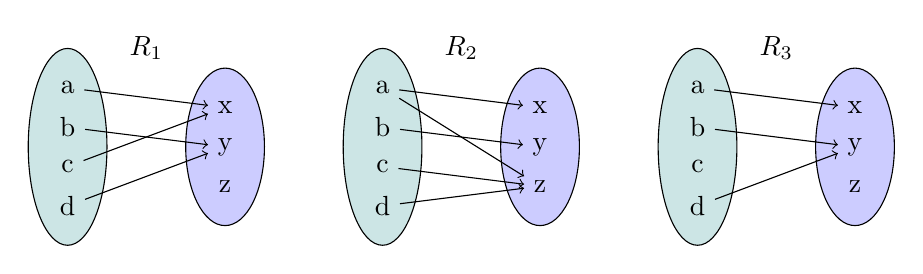
\begin{tikzpicture}[scale = 0.5]
\filldraw[fill = teal!20!white] (1,2.5) ellipse [x radius = 1, y radius = 2.5];
\filldraw[fill = blue!20!white] (5,2.5) ellipse [x radius = 1, y radius = 2];
\node at (1,4) (a1) {a};
\node at (1,3) (a2) {b};
\node at (1,2) (a3) {c};
\node at (1,1) (a4) {d};
\node at (5,3.5) (b1) {x};
\node at (5,2.5) (b2) {y};
\node at (5,1.5) (b3) {z};
\draw[->] (a1) -- (b1);
\draw[->] (a2) -- (b2);
\draw[->] (a3) -- (b1);
\draw[->] (a4) -- (b2);
\node at (3,5) {$R_1$};
\begin{scope}[xshift = 8cm]
\filldraw[fill = teal!20!white] (1,2.5) ellipse [x radius = 1, y radius = 2.5];
\filldraw[fill = blue!20!white] (5,2.5) ellipse [x radius = 1, y radius = 2];
\node at (1,4) (a1) {a};
\node at (1,3) (a2) {b};
\node at (1,2) (a3) {c};
\node at (1,1) (a4) {d};
\node at (5,3.5) (b1) {x};
\node at (5,2.5) (b2) {y};
\node at (5,1.5) (b3) {z};
\draw[->] (a1) -- (b1);
\draw[->] (a1) -- (b3);
\draw[->] (a2) -- (b2);
\draw[->] (a3) -- (b3);
\draw[->] (a4) -- (b3);
\node at (3,5) {$R_2$};
\end{scope}
\begin{scope}[xshift = 16cm]
\filldraw[fill = teal!20!white] (1,2.5) ellipse [x radius = 1, y radius = 2.5];
\filldraw[fill = blue!20!white] (5,2.5) ellipse [x radius = 1, y radius = 2];
\node at (1,4) (a1) {a};
\node at (1,3) (a2) {b};
\node at (1,2) (a3) {c};
\node at (1,1) (a4) {d};
\node at (5,3.5) (b1) {x};
\node at (5,2.5) (b2) {y};
\node at (5,1.5) (b3) {z};
\draw[->] (a1) -- (b1);
\draw[->] (a2) -- (b2);
\draw[->] (a4) -- (b2);
\node at (3,5) {$R_3$};
\end{scope}
\end{tikzpicture}
\caption{Which ones are functions?}
\end{figure}
\end{frame}


\begin{frame}
\begin{sol}
\begin{itemize}
\item $R_1$ is a function, because each element on the left has exactly one out arrow.
\item $R_2$ is not a function, because there are two arrows going out from $a$.
\item $R_3$ is not a function, because there are no arrows going out from $c$.
\end{itemize}

\begin{figure}[h!]
\centering
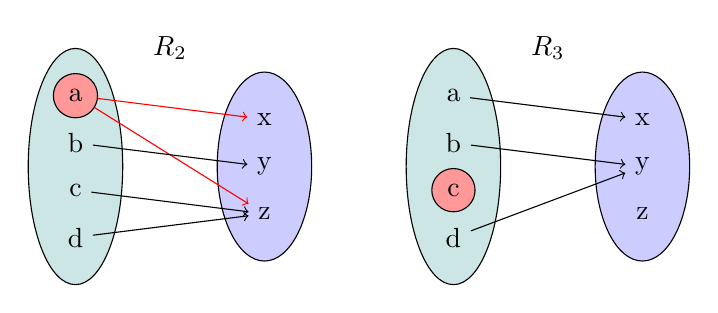
\begin{tikzpicture}[scale = 0.6]
\filldraw[fill = teal!20!white] (1,2.5) ellipse [x radius = 1, y radius = 2.5];
\filldraw[fill = blue!20!white] (5,2.5) ellipse [x radius = 1, y radius = 2];
\node[draw, circle, fill = red!40] at (1,4) (a1) {a};
\node at (1,3) (a2) {b};
\node at (1,2) (a3) {c};
\node at (1,1) (a4) {d};
\node at (5,3.5) (b1) {x};
\node at (5,2.5) (b2) {y};
\node at (5,1.5) (b3) {z};
\draw[->, red] (a1) -- (b1);
\draw[->, red] (a1) -- (b3);
\draw[->] (a2) -- (b2);
\draw[->] (a3) -- (b3);
\draw[->] (a4) -- (b3);
\node at (3,5) {$R_2$};
\begin{scope}[xshift = 8cm]
\filldraw[fill = teal!20!white] (1,2.5) ellipse [x radius = 1, y radius = 2.5];
\filldraw[fill = blue!20!white] (5,2.5) ellipse [x radius = 1, y radius = 2];
\node at (1,4) (a1) {a};
\node at (1,3) (a2) {b};
\node[draw, circle, fill = red!40] at (1,2) (a3) {c};
\node at (1,1) (a4) {d};
\node at (5,3.5) (b1) {x};
\node at (5,2.5) (b2) {y};
\node at (5,1.5) (b3) {z};
\draw[->] (a1) -- (b1);
\draw[->] (a2) -- (b2);
\draw[->] (a4) -- (b2);
\node at (3,5) {$R_3$};
\end{scope}
\end{tikzpicture}
\caption{Solutions}
\end{figure}
\end{sol}
\end{frame}

\begin{frame}
\frametitle{How to Test If It's a Function (2)}
If expressed as a graph, every vertical line must intersect the graph once.

\begin{figure}[h!]
\centering
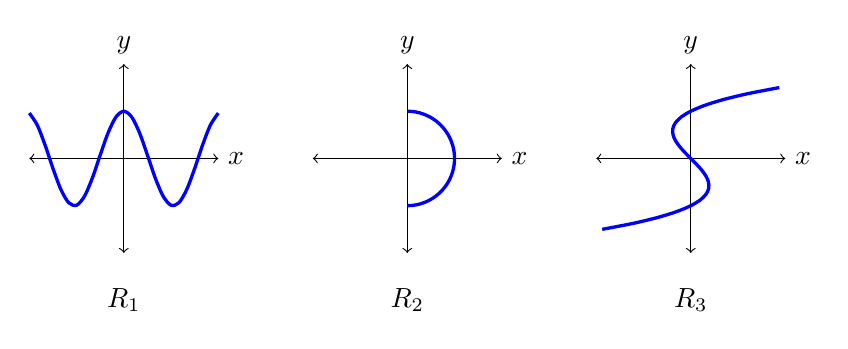
\begin{tikzpicture}[scale = 0.6, smooth]
\axes{-2}{2}{-2}{2};
\draw[blue, very thick, domain = -2:2] plot (\x, {cos(\x*3 r)});
\node at (0,-3) {$R_1$};
\begin{scope}[xshift = 6cm]
\axes{-2}{2}{-2}{2};
\draw[blue, variable = \t, very thick, domain = {-pi/2}:{pi/2}] plot ({cos(\t r)},{sin(\t r)});
\node at (0,-3) {$R_2$};
\end{scope}
\begin{scope}[xshift = 12cm]
\axes{-2}{2}{-2}{2};
\draw[blue, variable = \t, very thick, domain = -1.5:1.5] plot ({\t^3-\t},{\t});
\node at (0,-3) {$R_3$};
\end{scope}
\end{tikzpicture}
\caption{Which ones are functions?}
\end{figure}
\end{frame}


\begin{frame}
\begin{sol}
\begin{itemize}
\item $R_1$ is a function, because any vertical line intersects the function at most once.
\item $R_2$ is not a function, because there is a vertical line that intersects the graph twice.
\item $R_3$ is not a function, because there is a vertical line that intersects the graph twice.
\end{itemize}

\begin{figure}[h!]
\centering
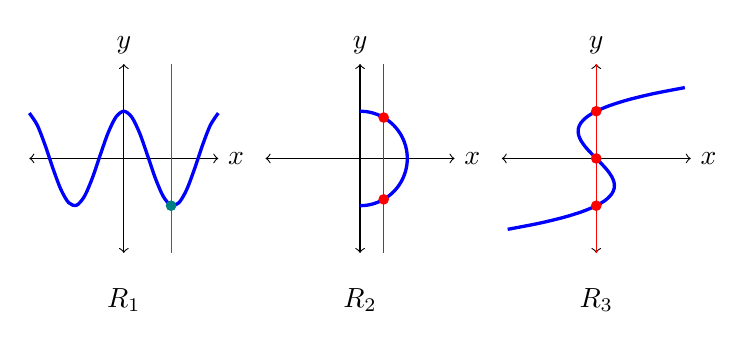
\begin{tikzpicture}[scale = 0.6, smooth]
\axes{-2}{2}{-2}{2};
\draw[color=blue, very thick, domain = -2:2] plot (\x, {cos(\x*3 r)});
\node at (0,-3) {$R_1$};
\draw[teal] (1,-2) --+ (0,4);
\filldraw[teal] (1,-1) circle [radius = 0.1cm];
\begin{scope}[xshift = 5cm]
\axes{-2}{2}{-2}{2};
\draw[color=blue, variable = \t, very thick, domain = {-pi/2}:{pi/2}] plot ({cos(\t r)},{sin(\t r)});
\node at (0,-3) {$R_2$};
\draw[red] (0.5,-2) --+ (0,4) ;
\filldraw[red] (0.5,{sqrt(3)/2}) circle [radius = 0.1cm];
\filldraw[red] (0.5,{-sqrt(3)/2}) circle [radius = 0.1cm];
\end{scope}
\begin{scope}[xshift = 10cm]
\axes{-2}{2}{-2}{2};
\draw[color=blue, variable = \t, very thick, domain = -1.5:1.5] plot ({\t^3-\t},{\t});
\node at (0,-3) {$R_3$};
\draw[red] (0,-2) --+ (0,4) ;
\filldraw[red] (0,-1) circle [radius = 0.1cm];
\filldraw[red] (0,0) circle [radius = 0.1cm];
\filldraw[red] (0,1) circle [radius = 0.1cm];
\end{scope}
\end{tikzpicture}
\caption{Graph for example \theexample}
\end{figure}
\end{sol}
\end{frame}

\iffalse
\begin{frame}
\begin{exercisebox}{}
Convert the following sentence in to functions in all 5 ways.
\begin{enumerate}
\item $f(x) = x+2$
\item $f(x) = x^2$
\end{enumerate}
\end{exercisebox}
\end{frame}
\fi

\iffalse
%%%%%%%%%%%%%
\section{Let's Cooperate!}
\frame{\sectionpage}
%%%%%%%%%%%%%

% classic Battleship
\begin{frame}
\begin{figure}[h!]
\centering

\includegraphics[width = 0.7\textwidth]{l07i15.png}
\caption{Battleship (1967)}
\end{figure}
\end{frame}

\begin{frame}
\begin{figure}[h!]
\centering

\includegraphics[width = 0.5\textwidth]{l07i16.png}
\caption{Sonar (2018)}
\end{figure}
\end{frame}
\fi

%%%%%%%%%%%%%
\section[Evaluation]{Function Evaluation}
\frame{\sectionpage}
%%%%%%%%%%%%%


\begin{frame}[t]
\frametitle{Function evaluation}
Given a function $f$ and a real number $a$ in the domain, we can define $f(a)$ to be the value when we substitute $x=a$ in the function. In other words, we replace all occurences of $x$ by $a$ \pa

\begin{ex}
Let $f(x) = 2x+1$. Compute the followings.
\begin{tasks}(4)
\task $f(0)$
\task $f(1)$
\task $f(0.5)$ 
\task $f(100)$
\end{tasks}
\end{ex}
\begin{sol}
\begin{eqnarray*} 
\mbox{When } x=0 &\mbox{ we have }& \pa f(0) = 2(0) + 1 \pa = 1 \\ \pa
\mbox{When } x=1 &\mbox{ we have }& \pa f(1) = 2(1) + 1 \pa = 2+1 \pa = 3\\ \pa
\mbox{When } x=0.5 &\mbox{ we have }& \pa f(0.5) = 2(0.5) + 1 \pa = 1 + 1 \pa = 2\\ \pa
\mbox{When } x=100 &\mbox{ we have }& \pa f(100) = 2(100) + 1 \pa = 200 + 1 \pa = 201
\end{eqnarray*}
\end{sol}
\end{frame}


\begin{frame}[t]
\begin{ex}
Let $f(x) = x^2+x$. Compute the followings.
\begin{tasks}(4)
\task $f(0)$
\task $f(2)$
\task $f(-3)$ 
\task $f\left(\frac{1}{3}\right)$
\end{tasks}
\end{ex}
\begin{sol}
\begin{tasks}(1)
\task $f(0) \pa = 0^2 + 0 = 0$ \pa
\task $f(2) \pa = 2^2 + 2 \pa= 4+2 \pa= 6$ \pa
\task $f(-3) \pa = (-3)^2 + (-3) \pa = 9 - 3 \pa = 6$ \pa
\task $f\left(\frac{1}{3}\right) \pa= \left(\frac{1}{3}\right)^2 + \frac{1}{3} \pa= \frac{1}{9} + \frac{1}{3} \pa= \frac{4}{9}$
\end{tasks}
\end{sol}
\end{frame}

\begin{frame}[t]
\frametitle{Remarks}
\begin{remark}{}
We don't need to let $x$ be a number. It can be \textbf{anything}. For instance, let $f(x) = x^2+3x$. Then, we can write the followings.
\begin{slide}
\begin{eqnarray*}
f(y) &=& y^2+3y \\ \pa
f(\Xi) &=& \Xi^2 + 3\Xi \\ \pa
f(x+5) &=& (x+5)^2 + 3(x+5) \\ \pa
f(x+h) &=& (x+h)^2 + 3(x+h) \\ \pa
f\left(\frac{1}{x}\right) &=& \left(\frac{1}{x}\right)^2 + 3\left(\frac{1}{x}\right) \pa
\end{eqnarray*}
\end{slide}
\end{remark}
\end{frame}

\begin{frame}
\begin{exercisebox}{}
1. Google for your favorite/cool looking/bizarre/cute/funny graph.
\begin{figure}[h!]
\centering

\includegraphics[width = 0.7\textwidth]{l07i20.png}
\caption{\href{desmos.com/calculator}{Desmos.com}}
\end{figure}
\end{exercisebox}
\end{frame}

%%%%%%%%%%%%%
\section[Algebra]{Algebra of Functions}
\frame{\sectionpage}
%%%%%%%%%%%%%

\begin{frame}
\frametitle{Algebra of Functions}
Algebra of functions is the operation of the functions, specifically the arithematic operations.
\begin{prop}{}{}
Let $f$ and $g$ be functions and $c$ be a constant.
\begin{enumerate}
\item $(cf) (x) = c ( f(x) )$ \pa
\item $(f+g) (x) = f(x) + g(x)$ \pa
\item $(f-g) (x) = f(x) - g(x)$
\item $(f \cdot g) (x) = f(x) \cdot g(x) $
\item $ \left(\frac{f}{g}\right)(x) = \frac{f(x)}{g(x)}$ where $g(x) \neq 0$
\end{enumerate}
\end{prop}
\end{frame}


\begin{frame}[t]
\begin{ex}
Let $f(x) = x+1$ and $g(x) = 2x-3$. Find the followings.
\begin{tasks}(4)
\task $(2f)(x)$
\task $(f+g)(x)$ 
\task $(f - g)(x)$
\task $(3f + 2g)(x)$
\end{tasks}
\end{ex}
\begin{sol}
\begin{eqnarray*}
(2f)(x) \pa &=& 2f(x)  \\ \pa
&=& 2(x+1) \pa = 2x+2 \\ \pa
(f+g)(x) \pa &=& (x+1) + (2x-3)  \\ \pa
&=& (x+2x) + (1-3) \pa = 3x-2 \\ \pa
(f-g)(x) \pa &=& (x+1) - (2x-3) \\ \pa
&=& (x+1) + (-2x + 3) \pa = (x-2x) + (1+3) \pa = -x+4 \\ \pa
(3f + 2g) &=& 3f(x) + 2g(x) \\ \pa
&=& 3(x+1) + 2(2x-3) \pa = (3x+3) + (4x-6) \pa = (7x-3)
\end{eqnarray*}
\end{sol}
\end{frame}


\begin{frame}[t]
\begin{ex}
Let $f(x) = x+1$ and $g(x) = 2x-3$. Find the followings.
\begin{tasks}(2)
\task $(fg)(x)$
\task $\left( \frac{f}{g} \right)(x)$
\end{tasks}
\end{ex}
\begin{sol}
\begin{eqnarray*}
(fg)(x) \pa &=& (x+1)(2x-3) \\ \pa
&=& 2x^2-3x+2x-3 \pa = 2x^2-x-3\\ \pa
\left(\frac{f}{g} \right)(x)&=& \frac{x+1}{2x-3}
\end{eqnarray*}
We can leave the fraction as is.
\end{sol}
\end{frame}


%%%%%%%%%%%%%%
\section[Composite]{Composite Function}
\frame{\sectionpage}
%%%%%%%%%%%%%%

\begin{frame}
\frametitle{Example of a composite system}
\addfig{0.8}{function_intro_factori}{A chain of factories \href{https://www.youtube.com/watch?v=v-tFGm9nCV0&ab_channel=StarGardenGames}{(Source)}}{}
\end{frame}


\begin{frame}{composite function}
We can combite two (or more) functions by chaining them.
\begin{defn}{}{}
Let $f(x)$ and $g(x)$ be functions. A composite function, denoted $f \circ g$, is defined as
 \[ (f \circ g)(x)= f(g(x))\]
In other words, we replace $x$ in $f(x)$ by another function $g(x)$.
\end{defn}
\end{frame}

\begin{frame}
\begin{figure}[h!]
\centering
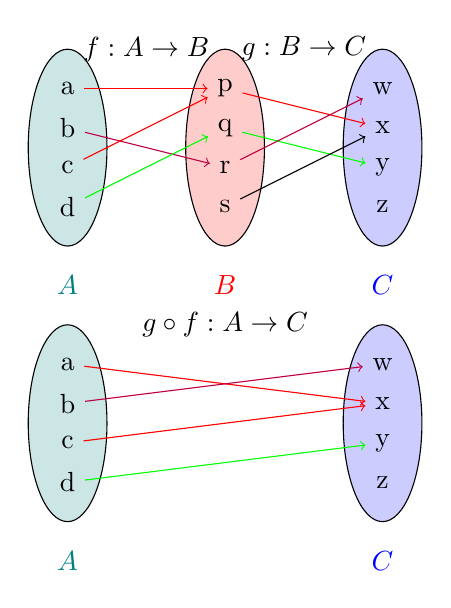
\begin{tikzpicture}[scale = 0.5]
\filldraw[fill = teal!20!white] (1,2.5) ellipse [x radius = 1, y radius = 2.5];
\node[teal] at (1,-1) {$A$};
\filldraw[fill = red!20!white] (5,2.5) ellipse [x radius = 1, y radius = 2.5];
\node[red] at (5,-1) {$B$};
\filldraw[fill = blue!20!white] (9,2.5) ellipse [x radius = 1, y radius = 2.5];
\node[blue] at (9,-1) {$C$};
\node at (1,4) (a1) {a};
\node at (1,3) (a2) {b};
\node at (1,2) (a3) {c};
\node at (1,1) (a4) {d};
\node at (5,4) (b1) {p};
\node at (5,3) (b2) {q};
\node at (5,2) (b3) {r};
\node at (5,1) (b4) {s};
\node at (9,4) (c1) {w};
\node at (9,3) (c2) {x};
\node at (9,2) (c3) {y};
\node at (9,1) (c4) {z};
\draw[->, red] (a1) -- (b1);
\draw[->, purple] (a2) -- (b3);
\draw[->, red] (a3) -- (b1);
\draw[->, green] (a4) -- (b2);
\draw[->, red] (b1) -- (c2);
\draw[->, green] (b2) -- (c3);
\draw[->, purple] (b3) -- (c1);
\draw[->] (b4) -- (c2);
\node at (3, 5) {$f: A \rightarrow B$};
\node at (7, 5) {$g: B \rightarrow C$};
\begin{scope}[yshift = -7cm]
\filldraw[fill = teal!20!white] (1,2.5) ellipse [x radius = 1, y radius = 2.5];
\node[teal] at (1,-1) {$A$};
\filldraw[fill = blue!20!white] (9,2.5) ellipse [x radius = 1, y radius = 2.5];
\node[blue] at (9,-1) {$C$};
\node at (1,4) (a1) {a};
\node at (1,3) (a2) {b};
\node at (1,2) (a3) {c};
\node at (1,1) (a4) {d};
\node at (9,4) (c1) {w};
\node at (9,3) (c2) {x};
\node at (9,2) (c3) {y};
\node at (9,1) (c4) {z};
\draw[->, red] (a1) -- (c2);
\draw[->, purple] (a2) -- (c1);
\draw[->, red] (a3) -- (c2);
\draw[->, green] (a4) -- (c3);
\node at (5, 5) {$g\circ f: A \rightarrow C$};
\end{scope}
\end{tikzpicture}
\caption{Creating the composite function $g \circ f$ using set diagram}
\end{figure}
\end{frame}

\begin{frame}
\begin{figure}[h!]
\centering
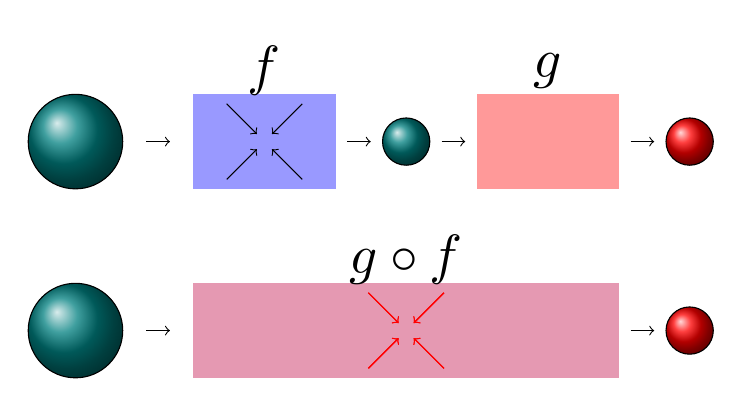
\begin{tikzpicture}[scale = 0.6]
\filldraw[blue!40] (0,0) rectangle (3,2);
\foreach \x in {-0.8,0.8}
{
	\foreach \y in {-0.8,0.8}
	{
		\draw[->] ({1.5+\x}, {1+\y}) -- ({1.5+(0.2*\x)},{1+(0.2*\y)});
	}
}
\filldraw[red!40] (6,0) rectangle (9,2);
\filldraw[ball color = teal] (-2.5,1) circle [radius = 1cm];
\filldraw[ball color = teal] (4.5,1) circle [radius = 0.5cm];
\filldraw[ball color = red] (10.5,1) circle [radius = 0.5cm];
\foreach \x in {-1, 3.25, 5.25, 9.25}
{
	\draw[->] (\x,1) -- ({\x+0.5},1);
}
\node[scale = 2] at (1.5, 2.5) {$f$};
\node[scale = 2] at (7.5, 2.5) {$g$};
\begin{scope}[yshift = -4cm]
\filldraw[purple!40] (0,0) rectangle (9,2);
\foreach \x in {-1,1}
\foreach \x in {-0.8,0.8}
{
	\foreach \y in {-0.8,0.8}
	{
		\draw[->, red] ({4.5+\x}, {1+\y}) -- ({4.5+(0.2*\x)},{1+(0.2*\y)});
	}
}
\filldraw[ball color = teal] (-2.5,1) circle [radius = 1cm];
\filldraw[ball color = red] (10.5,1) circle [radius = 0.5cm];
\foreach \x in {-1, 9.25}
{
	\draw[->] (\x,1) -- ({\x+0.5},1);
}
\node[scale = 2] at (4.5, 2.5) {$g \circ f$};
\end{scope}
\end{tikzpicture}
\caption{Creating a composite function as a chain of machines}
\end{figure}
\end{frame}

\begin{frame}
\addfig{0.7}{function_composite_meme1}{The difference between $f \circ g$ and $g \circ f$}{}
\end{frame}


\begin{frame}[t]
\begin{ex}
Let $f(x) = x+1$ and $g(x) = x^2$. Find the followings.
\begin{tasks}(2)
\task $(f \circ g)(x)$
\task $(g \circ f)(x)$
\task $(f \circ f)(x)$
\task $(g \circ g)(x)$
\end{tasks}
\end{ex}
\begin{sol}
\begin{eqnarray*}
(f \circ g)(x) \pa &=& f(\alert{g(x)}) \pa= \alert{g(x)} + 1 = x^2 + 1 \\ \pa
(g \circ f)(x) \pa &=& g(\green{f(x)}) \pa = \green{f(x)}^2 \pa = \green{(x+1)}^2
\end{eqnarray*}
Notice that $(f \circ g)(x) \neq (g \circ f)(x)$, so the order matters.
\begin{eqnarray*}
(f \circ f)(x) \pa &=& f(\green{f(x)}) \pa = \green{f(x)} + 1 \pa = \green{x+1} + 1 \pa = x+2 \\ \pa
(g \circ g)(x) \pa &=& g(\red{g(x)}) \pa = (\red{g(x)})^2 \pa = (\red{x^2})^2 \pa = x^4
\end{eqnarray*}
\end{sol}
\end{frame} 


\begin{frame}[t]
\begin{ex}
Let $f(x) = \sqrt{x} $ and $g(x) = 2x+1$. Find the followings.
\begin{tasks}(2)
\task $(f \circ g)(x)$
\task $(f \circ g)(4)$
\task $(g \circ f)(x)$
\task $(g \circ f)(4)$
\end{tasks}
\end{ex}
\begin{sol}
\begin{eqnarray*}
(f \circ g)(x) \pa &=& f(\alert{g(x)}) \pa= \sqrt{\alert{g(x)}} \pa = \sqrt{2x+1} \\ \pa
(f \circ g)(4) \pa &=& \sqrt{2(4) + 1 } \pa = \sqrt{9} \pa = 3 \\ \pa
(g \circ f)(x) \pa &=& g(\green{f(x)}) \pa = 2\green{f(x)}+1 \pa = 2\green{\sqrt{x}} + 1 \\ \pa
(g \circ f)(4) \pa &=& 2\sqrt{4} + 1 \pa =  2(2) + 1 \pa = 5
\end{eqnarray*}
\end{sol}
\end{frame}

\iffalse
%%%%%%%%%%%%%%
\section{ฟังก์ชันผกผัน}
\frame{\sectionpage}
%%%%%%%%%%%%%%

\begin{frame}
\frametitle{นิยามฟังก์ชันหนึ่งต่อหนึ่ง}
ก่อนจะนิยามฟังก์ชันผกผันได้ เราจะต้องนิยามฟังก์ชันหนึ่งต่อหนึ่งก่อน
\begin{defn}{}{}
$f: A \rightarrow B$ เป็นฟังก์ชันหนึ่งต่อหนึ่ง ก็ต่อเมื่อ ไม่มีคู่อันดับที่สมาชิกตัวหลังเหมือนกัน \textbf{แต่สมาชิกตัวหน้าต่างกัน}
\end{defn} \pa

เช่น $f = \{ (1,A), (2,B), (3,C)\}$ เป็นฟังก์ชัน 1 ต่อ 1 \pa

$g = \{(1,A), (2,A), (3,B)\}$ ไม่เป็นฟังก์ชัน 1 ต่อ 1 เพราะ $(1,A), (2,A)$ มีสมาชิกตัวหลังเหมือนกันแต่ตัวหน้าต่างกัน \pa
\end{frame}

\begin{frame}
\begin{figure}[h!]
\centering
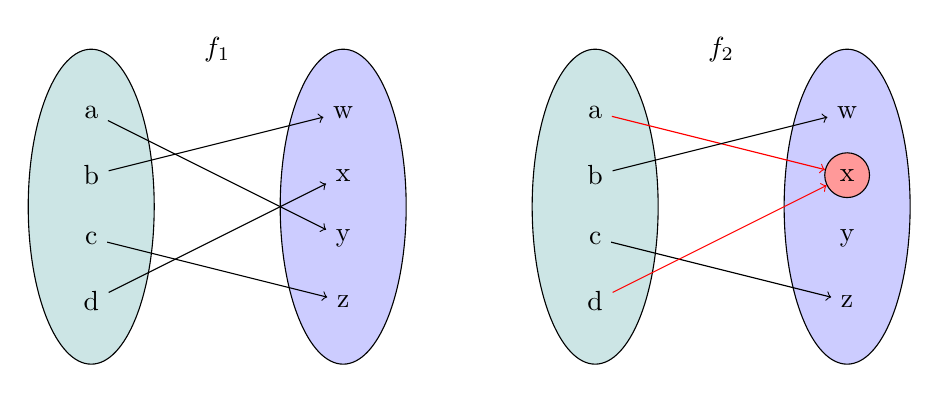
\begin{tikzpicture}[scale = 0.8]
\filldraw[fill = teal!20!white] (1,2.5) ellipse [x radius = 1, y radius = 2.5];
\filldraw[fill = blue!20!white] (5,2.5) ellipse [x radius = 1, y radius = 2.5];
\node at (1,4) (a1) {a};
\node at (1,3) (a2) {b};
\node at (1,2) (a3) {c};
\node at (1,1) (a4) {d};
\node at (5,4) (b1) {w};
\node at (5,3) (b2) {x};
\node at (5,2) (b3) {y};
\node at (5,1) (b4) {z};
\draw[->] (a1) -- (b3);
\draw[->] (a2) -- (b1);
\draw[->] (a3) -- (b4);
\draw[->] (a4) -- (b2);
\node at (3,5) {$f_1$};
\begin{scope}[xshift = 8cm]
\filldraw[fill = teal!20!white] (1,2.5) ellipse [x radius = 1, y radius = 2.5];
\filldraw[fill = blue!20!white] (5,2.5) ellipse [x radius = 1, y radius = 2.5];
\node at (1,4) (a1) {a};
\node at (1,3) (a2) {b};
\node at (1,2) (a3) {c};
\node at (1,1) (a4) {d};
\node at (5,4) (b1) {w};
\node[draw, circle, fill = red!40] at (5,3) (b2) {x};
\node at (5,2) (b3) {y};
\node at (5,1) (b4) {z};
\draw[->,red] (a1) -- (b2);
\draw[->] (a2) -- (b1);
\draw[->] (a3) -- (b4);
\draw[->,red] (a4) -- (b2);
\node at (3,5) {$f_2$};
\end{scope}
\end{tikzpicture}
\caption{ตัวอย่างฟังก์ชันหนึ่งต่อหนึ่ง $f_1$ และฟังก์ชันที่ไม่ใช่ฟังก์ชันหนึ่งต่อหนึ่ง $f_2$}
\end{figure}
\end{frame}

\begin{frame}
\frametitle{นิยามฟังก์ชันผกผัน}
\begin{defn}{}{}
กำหนดให้ $f$ เป็นฟังก์ชัน 1 ต่อ 1 \textbf{ ฟังก์ชันผกผันของ } $\mathbf{f}$ (เขียนแทนด้วย $f^{\, -1}$) คือฟังก์ชันที่มีสมบัติว่า
\[\text{ถ้า } y = f(x) \text{ แล้ว }f^{\, -1}(y) = x\]
\end{defn}
\end{frame}

\begin{frame}
ถ้ากำหนดฟังก์ชัน $f$ ในรูปแบบเซต เราสามารถสร้างฟังก์ชันผกผันได้ด้วยการสลับตำแหน่งเซต $A$ และ $B$ แล้วทำการสลับทิศทางลูกศรทั้งหมด

\begin{figure}[h!]
\centering
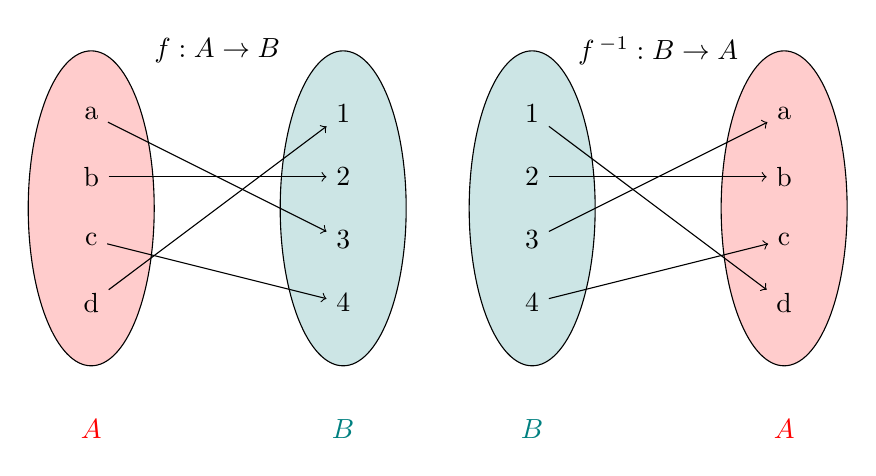
\begin{tikzpicture}[scale = 0.8]
\filldraw[fill = red!20!white] (1,2.5) ellipse [x radius = 1, y radius = 2.5];
\node[red] at (1,-1) {$A$};
\filldraw[fill = teal!20!white] (5,2.5) ellipse [x radius = 1, y radius = 2.5];
\node[teal] at (5,-1) {$B$};
\node at (1,4) (a1) {a};
\node at (1,3) (a2) {b};
\node at (1,2) (a3) {c};
\node at (1,1) (a4) {d};
\node at (5,4) (b1) {1};
\node at (5,3) (b2) {2};
\node at (5,2) (b3) {3};
\node at (5,1) (b4) {4};
\draw[->] (a1) -- (b3);
\draw[->] (a2) -- (b2);
\draw[->] (a3) -- (b4);
\draw[->] (a4) -- (b1);
\node at (3, 5) {$f: A \rightarrow B$};
\begin{scope}[xshift = 7cm]
\filldraw[fill = teal!20!white] (1,2.5) ellipse [x radius = 1, y radius = 2.5];
\node[teal] at (1,-1) {$B$};
\filldraw[fill = red!20!white] (5,2.5) ellipse [x radius = 1, y radius = 2.5];
\node[red] at (5,-1) {$A$};
\node at (5,4) (a1) {a};
\node at (5,3) (a2) {b};
\node at (5,2) (a3) {c};
\node at (5,1) (a4) {d};
\node at (1,4) (b1) {1};
\node at (1,3) (b2) {2};
\node at (1,2) (b3) {3};
\node at (1,1) (b4) {4};
\draw[<-] (a1) -- (b3);
\draw[<-] (a2) -- (b2);
\draw[<-] (a3) -- (b4);
\draw[<-] (a4) -- (b1);
\node at (3, 5) {$f\,^{-1}: B \rightarrow A$};
\end{scope}
\end{tikzpicture}
\caption{การสร้างฟังก์ชันผกผัน $f\,^{-1}$ ในรูปแบบความสัมพันธ์}
\end{figure}
\end{frame}

\begin{frame}
ถ้ากำหนดฟังก์ชัน $f$ ในรูปแบบการทำงานของเครื่องจักร เราสามารถสร้างฟังก์ชันผกผันได้ด้วยการหาว่าการทำงานแบบใดที่มีผลลัพธ์ตรงกันข้ามกับ $f$ เช่น ถ้า $f$ คือการลดขนาด แล้ว $f\,^{-1}$ คือการเพิ่มขนาด

\begin{figure}[h!]
\centering
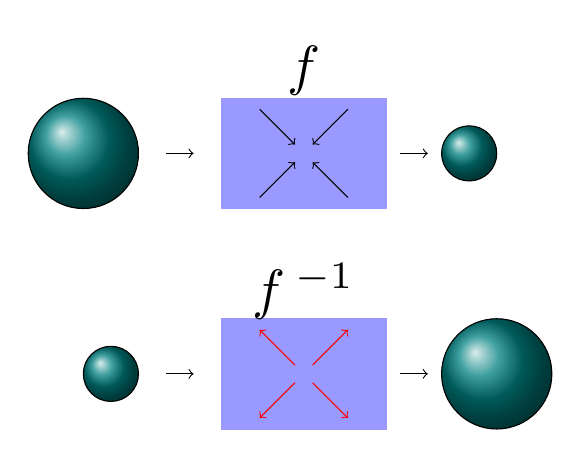
\begin{tikzpicture}[scale = 0.7]
\filldraw[blue!40] (0,0) rectangle (3,2);
\foreach \x in {-0.8,0.8}
{
	\foreach \y in {-0.8,0.8}
	{
		\draw[->] ({1.5+\x}, {1+\y}) -- ({1.5+(0.2*\x)},{1+(0.2*\y)});
	}
}
\filldraw[ball color = teal] (-2.5,1) circle [radius = 1cm];
\filldraw[ball color = teal] (4.5,1) circle [radius = 0.5cm];
\foreach \x in {-1, 3.25}
{
	\draw[->] (\x,1) -- ({\x+0.5},1);
}
\node[scale = 2] at (1.5, 2.5) {$f$};
\begin{scope}[yshift = -4cm]
\filldraw[blue!40] (0,0) rectangle (3,2);
\foreach \x in {-0.8,0.8}
{
	\foreach \y in {-0.8,0.8}
	{
		\draw[<-, red] ({1.5+\x}, {1+\y}) -- ({1.5+(0.2*\x)},{1+(0.2*\y)});
	}
}
\filldraw[ball color = teal] (-2,1) circle [radius = 0.5cm];
\filldraw[ball color = teal] (5,1) circle [radius = 1cm];
\foreach \x in {-1, 3.25}
{
	\draw[->] (\x,1) -- ({\x+0.5},1);
}
\node[scale = 2] at (1.5, 2.5) {$f\,^{-1}$};
\end{scope}
\end{tikzpicture}
\caption{การสร้างฟังก์ชันผกผัน $f\,^{-1}$ ในรูปการทำงานของเครื่องจักร}
\end{figure}
\end{frame}

\begin{frame}
ถ้ากำหนดฟังก์ชัน $f$ ในรูปแบบกราฟ เราสามารถสร้างฟังก์ชันผกผันได้ด้วยการแปลงจุด $(a,b)$ บนกราฟทั้งหมดให้กลายเป็นจุด $(b,a)$ ซึ่งมีค่าเท่ากับการสะท้อนกราฟฟังก์ชัน $y=f(x)$ บนเส้นแทยงมุม $y=x$ 

\begin{figure}[h!]
\centering
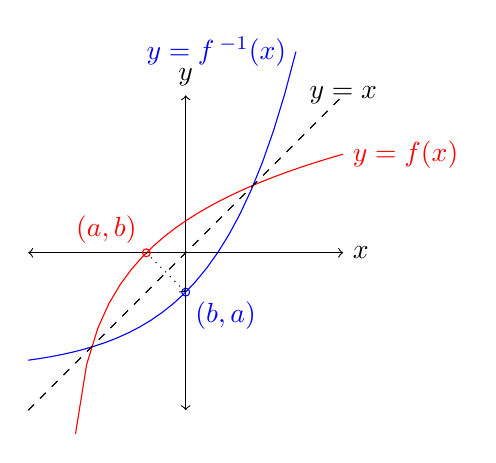
\begin{tikzpicture}
\axes{-2}{2}{-2}{2};
\draw[blue] plot[domain = -2:1.4] (\x, {exp(\x)-1.5}) node[left] {$y=f\,^{-1}(x)$};
\draw[red] plot[domain = -1.4:2] (\x, {ln(\x+1.5)}) node[right] 
{$y=f(x)$};
\draw[dashed] (-2,-2) -- (2,2) node {$y=x$};
\draw[red] (-0.5, 0) circle [radius = 0.05cm] node [above left] {$(a,b)$};
\draw[blue] (0, -0.5) circle [radius = 0.05cm] node [below right] {$(b,a)$};
\draw[dotted, ->] (-0.5,0) -- (0,-0.5);
\end{tikzpicture}
\caption{ตัวอย่างการหาฟังก์ชันผกผันจากกราฟ}
\end{figure}
\end{frame}

\begin{frame}
\addfig{0.6}{function_inverse_meme}{ภาพ meme เปรียบเทียบฟังก์ชันปกติ และฟังก์ชันผกผัน}{}
\end{frame}

\begin{frame}
\frametitle{วิธีหาฟังก์ชันผกผัน}
\begin{block}{}
\begin{enumerate}
\item กำหนดตัวแปร $y$ โดยที่ $y = f(x)$  \pa
\item สลับตัวแปรใหม่ ให้อยู่ในรูป $x = f(y)$ \pa
\item จัดรูปสมการให้ฝั่งซ้ายมี $y$ พจน์เดียว และฝั่งขวามีพจน์ $x$ และค่าคงตัวทั้งหมด \pa
\item สมการที่ได้จะอยู่ในรูป $y = f^{\, -1}$ ซึ่งเป็นฟังก์ชันผกผันที่ต้องการ
\end{enumerate}
\end{block}
\end{frame}


\begin{frame}[t]
\begin{ex}
กำหนดให้ $f(x) = x+2$ จงหา $f^{\, -1}(x)$
\end{ex}
\begin{sol}
\begin{itemize}
\item ขั้นแรกกำหนดตัวแปร $y = f(x)$ ขึ้นมาใหม่ \pa จะได้ 
\[y = x+2\] \pa
\item จากนั้นสลับตัวแปรใหม่จะได้เป็น \pa
\[x = y+2\] \pa
\item จัดรูปให้ $y$ อยู่ฝั่งซ้าย \pa จะได้
\[y = x-2\] \pa 
นั่นคือ $f^{-1}\,(x) = x-2$ เป็นฟังก์ชันผกผันที่ต้องการ
\end{itemize}
\end{sol}
\end{frame}


\begin{frame}[t]
\begin{ex}
กำหนดให้ $f(x) = x^2-3$ โดยที่ $x \geq 0$ จงหา $f^{\, -1}(x)$
\end{ex}
\begin{sol}
\begin{itemize}
\item ขั้นแรกกำหนดตัวแปร $y = f(x)$ ขึ้นมาใหม่ \pa จะได้ 
\[y = x^2-3, \text{ โดยที่ } x \geq 0\] \pa
\item สลับตัวแปรเป็น \pa
\[x = y^2-3, \text{ โดยที่ } y \geq 0\] \pa
จากนั้นจัดรูปใหม่\pa จะได้ 
\[y^2 = x+3  \qquad \rightarrow \qquad y = \pm \sqrt{x+3}\]
\pa แต่เนื่องจากเรากำหนดโดเมนที่มีค่า $y \geq 0$ \pa ฉะนั้นเราจึงได้ $y = \sqrt{x+3}$ \pa นั่นคือเราได้ฟังก์ชันผกผันเป็น  $f^{\, -1}(x) = \sqrt{x+3}$
\end{itemize}
\end{sol}
\end{frame}

\begin{frame}[t]
\frametitle{สมบัติของฟังก์ชันผกผัน}
\begin{prop}{}{}
กำหนดให้ $f: A \to B$ เป็นฟังก์ชันหนึ่งต่อหนึ่ง $D_f$ และ $R_f$ เป็นโดเมนและเรนจ์ของฟังก์ชันตามลำดับ
\begin{enumerate}
\item $f^{-1}: R_f \to A$ และเป็นฟังก์ชันหนึ่งต่อหนึ่งเช่นกัน
\item $(f \circ f^{-1}) (x) = x$ สำหรับทุก $x$ ใน $R_f$
\item $(f^{-1} \circ f)(x) = x$ สำหรับทุก $x$ ใน $A$
\end{enumerate}
\end{prop}
เช่น จากตัวอย่างก่อนหน้านี้เราทราบว่า $f(x) = x^2-3$ และ $f^{-1}(x) = \sqrt{x+3}$ ฉะนั้น
\begin{slide}
\[(f \circ f^{-1})(x) \pa = f( f^{-1}(x)) \pa = f( \sqrt{x+3} ) \pa = \sqrt{x+3}^2 - 3 \pa = (x+3) - 3 = x\]
\end{slide}
\end{frame}
\fi

%%%%%%%%%%%%%
\section[Coordinate]{Coordinate System and Graph}
\frame{\sectionpage}
%%%%%%%%%%%%%

\begin{frame}
\begin{block}{Why do we plot graphs?}
\begin{itemize}
\item Visualize \pause 
\item Prediction, tendency, asymptotic \pause
\item Comparison \pause
\item Discover correlation \pause
\item Recreational purpose \pause
\end{itemize}
\end{block}

\begin{defn}{}{}
In geometry, a \textbf{coordinate system} is a system that uses one or more numbers, or coordinates, to uniquely determine the position of the points.
\end{defn}
\end{frame}

\begin{frame}
\begin{figure}[h!]
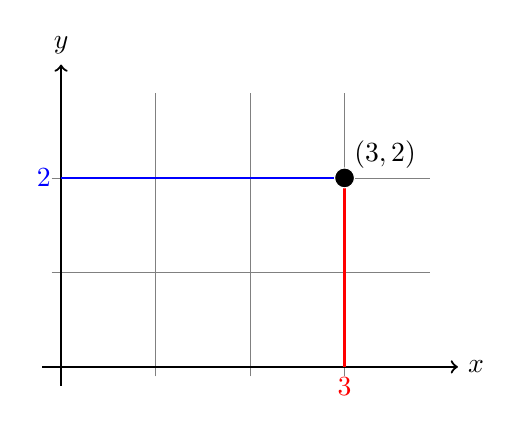
\begin{tikzpicture}[domain=0:4, scale = 1.2]
\draw[very thin,color=gray] (-0.1,-0.1) grid (3.9,2.9);
\draw[->, thick] (-0.2,0) -- (4.2,0) node[right] {$x$};
\draw[->, thick] (0,-0.2) -- (0,3.2) node[above] {$y$};
\draw[-, red, thick] (3,2) -- (3,0) node[below] {$3$};
\draw[-, blue, thick] (3,2) -- (0,2) node[left] {$2$};
\filldraw[fill = black, draw = white] (3,2) circle (3pt)
node [above right] {$(\red{3},\blue{2})$};
\end{tikzpicture}
\caption{A coordinate of $(x,y) = (3,2)$}
\end{figure}
\end{frame}

\begin{frame}
\begin{defn}{}{}
The \textbf{Cartesian coordinate system} is an coordinate system that specifies each point uniquely in a plane by a set of numerical coordinates. \pause
\end{defn}

\begin{block}{}
A graph of a function $f(x)$ shows a collection of points $(x, f(x))$ on the Cartesian plane.
\end{block}
\end{frame}

\begin{frame}
\begin{figure}[h!]
\centering

\includegraphics[width = 0.9\textwidth]{l07i20.png}
\caption{\href{desmos.com/calculator}{Online graphing utility}}
\end{figure}
\end{frame}



\begin{frame}[t]
\begin{ex}
Plot the points $(x,f(x))$ for the function $f(x) = x^2$ with $x=-2,-1,0,1,2$.
\end{ex}
\begin{sol}
\addfig{0.6}{graph_plot_ex1.png}{The plot of the function $f(x) = x^2$}{}
\end{sol}
\end{frame}


\begin{frame}[t]
\begin{ex}
Plot the points $(x,f(x))$ for the function $f(x) = \frac{1}{x^2+1}$ with $x=-2,-1,0,1,2$.
\end{ex}
\begin{sol}
\addfig{0.8}{graph_plot_ex2.png}{The plot of the function $f(x) = \frac{1}{x^2+1}$}{}
\end{sol}
\end{frame}


\begin{frame}[t]
\begin{ex}
Plot the points $(x,f(x))$ for the function $f(x) = | |x+1| - 1 |$ with $x=-2,-1,0,1,2$.
\end{ex}
\begin{sol}
\addfig{0.8}{graph_plot_ex3.png}{The plot of the function $f(x) = \frac{1}{x^2+1}$}{}
\end{sol}
\end{frame}


\begin{frame}
\begin{exercisebox}{}
Plot the points $(x,f(x))$ for the following functions with $x=-2,-1,0,1,2$ and connect the points to predict its shape.
\begin{enumerate}
\item $f(x) = \frac{x+1}{x+3}$
\item $f(x) = |2x+2|$
\item $f(x) = ||x|-1|$
\end{enumerate}
\end{exercisebox}
\end{frame}

%%%%%%%%%%%%%%
\section{Function Type}
\frame{\sectionpage}
%%%%%%%%%%%%%%

\begin{frame}
\frametitle{Basic Functions}
We will learn some basic functions.
\begin{enumerate}
\item Constant function
\item Linear function
\item Quadratic function
\item Polynomial function
\item Rational function
\item Absolute value function
\end{enumerate}
\end{frame}

\begin{frame}
\frametitle{1. Constant Function}
A constant function is of the form
\begin{block}{}\[f(x) = c\]\end{block} 
when $c$ is a constant. The graph is a horizontal line parallel to the x-axis. \pause
\textbf{Ex.}  $f(x) = -2, f(x) = 5$ \pause


\begin{figure}[h!]
\centering
\begin{tikzpicture}[scale = 0.5, smooth, domain = -2:2]
\axes{-2}{2}{-2}{2};
\draw[blue] plot (\x, 1.8);
\node[blue] at (0, -3) {$f(x) =4$};
\begin{scope}[xshift = 6cm]
\axes{-2}{2}{-2}{2};
\draw[red] plot (\x, 0.25);
\node[red] at (0,-3) {$f(x) = 0.5$};
\end{scope}
\begin{scope}[xshift = 12cm]
\axes{-2}{2}{-2}{2};
\draw[teal] plot (\x, -1);
\node[teal] at (0,-3) {$f(x) = -2$};
\end{scope}
\end{tikzpicture}
\caption{Constant functions $f(x) = c$}
\end{figure}
\end{frame}

\begin{frame}
\frametitle{2. Linear Function}
A linear function is of the form 
\begin{block}{}\[f(x) = ax+b\]\end{block} 
where $a,b$ are constants and $a \neq 0$. 
\textbf{Ex.} $f(x) = 2x, f(x) = -3x + 1$ \pause

\begin{figure}[h!]
\centering
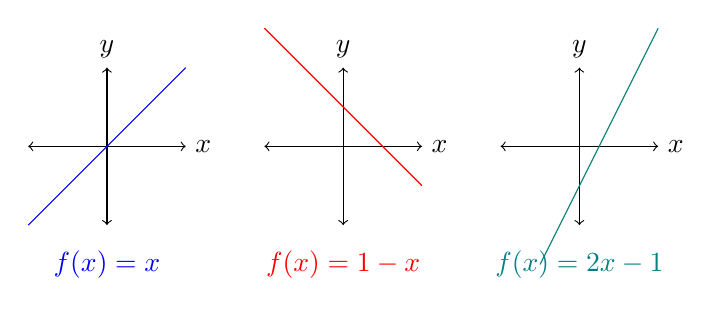
\begin{tikzpicture}[scale = 0.5, smooth, domain = -2:2]
\axes{-2}{2}{-2}{2};
\draw[blue] plot (\x, {\x});
\node[blue] at (0,-3) {$f(x) =x$};
\begin{scope}[xshift = 6cm]
\axes{-2}{2}{-2}{2};
\draw[red] plot (\x, {1-\x});
\node[red] at (0,-3) {$f(x) = 1-x$};
\end{scope}
\begin{scope}[xshift = 12cm]
\axes{-2}{2}{-2}{2};
\draw[teal] plot[domain = -1:2] (\x, {2*\x-1});
\node[teal] at (0,-3) {$f(x) = 2x-1$};
\end{scope}
\end{tikzpicture}
\caption{Linear functions $f(x) = ax+b$}
\end{figure}
\end{frame}

\begin{frame}
\frametitle{3. Quadratic Function}
A quadratic function is of the form
\begin{block}{}\[f(x) = ax^2+bx+c\]\end{block}
 when $a,b,c$ are constants and $a \neq 0$. The graph is called a \textbf{parabola}.

\textbf{Ex.} $f(x) = x^2+2x+3, f(x) = 5x^2 - 4$ \pause


\begin{figure}[h!]
\centering
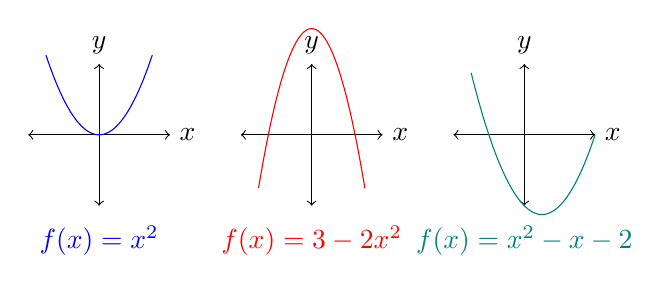
\begin{tikzpicture}[scale = 0.45, smooth, domain = -2:2]
\axes{-2}{2}{-2}{2};
\draw[blue] plot[domain = -1.5:1.5] (\x, {\x*\x});
\node[blue] at (0,-3) {$f(x) =x^2$};
\begin{scope}[xshift = 6cm]
\axes{-2}{2}{-2}{2};
\draw[red] plot[domain = -1.5:1.5] (\x, {3-2*(\x*\x)});
\node[red] at (0,-3) {$f(x) = 3-2x^2$};
\end{scope}
\begin{scope}[xshift = 12cm]
\axes{-2}{2}{-2}{2};
\draw[teal] plot[domain = -1.5:2] (\x, {(\x*\x)-\x-2});
\node[teal] at (0,-3) {$f(x) = x^2-x-2$};
\end{scope}
\end{tikzpicture}
\caption{Quadratic functions $f(x) = ax^2+bx+c$}
\end{figure}
\end{frame}

\begin{frame}
\frametitle{4. Polynomial Function}
A polynomial function (also called a polynomial) is of the form 
\begin{block}{}\[f(x) = a_n x^n + a_{n-1}x^{n-1} + \ldots + a_2 x^2 + a_1 x + a_0\] \end{block}
where $a_n, a_{n-1}, \ldots, a_2, a_1, a_0$ are all constants  and $n \geq 0$ is an integer. \pause


\begin{figure}[h!]
\centering
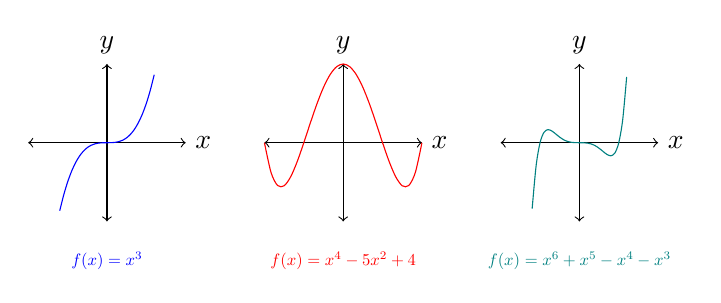
\begin{tikzpicture}[scale = 0.5, smooth, domain = -2:2]
\axes{-2}{2}{-2}{2};
\draw[blue] plot[domain = -1.2:1.2] (\x, {\x^3});
\node[blue, scale = 0.6] at (0,-3) {$f(x) =x^3$};
\begin{scope}[xshift = 6cm]
\axes{-2}{2}{-2}{2};
\draw[red] plot[domain = -2:2] (\x, {((\x*\x*\x*\x)-(5*(\x*\x))+4)/2});
\node[red, scale = 0.6] at (0,-3) {$f(x) = x^4-5x^2+4$};
\end{scope}
\begin{scope}[xshift = 12cm]
\axes{-2}{2}{-2}{2};
\draw[teal] plot[domain = -1.2:1.2] (\x, {(\x^6)+(\x^5)-(\x^4)-(\x^3)});
\node[teal, scale = 0.6] at (0,-3) {$f(x) = x^6+x^5-x^4-x^3$};
\end{scope}
\end{tikzpicture}
\caption{Polynomials $f(x) = a_nx^n + a_{n-1}x^{n-1} + \cdots + a_1x + a_0$}
\end{figure}
\end{frame}

\begin{frame}
\frametitle{5. Rational Function}
A rational function is of the form
\begin{block}{}\[f(x) = \frac{g(x)}{h(x)}\]\end{block}
where $g(x)$ and $h(x)$ are polynomials and $h(x)$ is not the constant function $h(x) = 0$. 

\textbf{Ex.} $\displaystyle f(x) = \frac{x+1}{x^2-1}, f(x) = \frac{4x^4 + 2x^2 + 1}{2x^2+1}, f(x) = \frac{1}{x^2+1}$ \pause

\begin{figure}[h!]
\centering
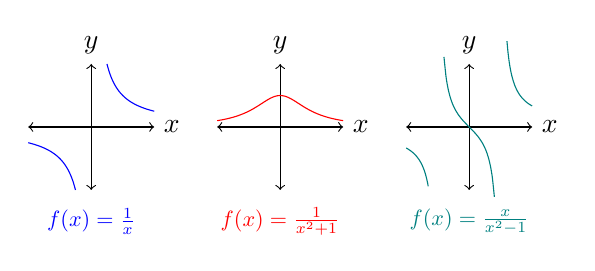
\begin{tikzpicture}[scale = 0.4, smooth, domain = -2:2]
\axes{-2}{2}{-2}{2};
\draw[blue] plot[domain = -2:-0.5] (\x, {1/\x});
\draw[blue] plot[domain = 0.5:2] (\x, {1/\x});
\node[blue, scale = 0.8] at (0,-3) {$f(x) = \frac{1}{x}$};
\begin{scope}[xshift = 6cm]
\axes{-2}{2}{-2}{2};
\draw[red] plot[domain = -2:2] (\x, {1/(\x*\x+1)});
\node[red, scale = 0.8] at (0,-3) {$f(x) = \frac{1}{x^2+1}$};
\end{scope}
\begin{scope}[xshift = 12cm]
\axes{-2}{2}{-2}{2};
\draw[teal] plot[domain = -2:-1.3] (\x, {(\x)/(\x*\x-1)});
\draw[teal] plot[domain = -0.8:0.8] (\x, {(\x)/(\x*\x-1)});
\draw[teal] plot[domain = 1.2:2] (\x, {(\x)/(\x*\x-1)});
\node[teal, scale = 0.8] at (0,-3) {$f(x) = \frac{x}{x^2-1}$};
\end{scope}
\end{tikzpicture}
\caption{Rational functions $f(x) = \tfrac{f(x)}{g(x)}$}
\end{figure}
\end{frame}


\begin{frame}
\frametitle{6. Absolute Value Function}
Recall that an absolute value is defined as
\begin{block}{}\[ |x| = \begin{cases} x &, \text{ if } x \geq 0 \\ -x &, \text{ if } x < 0\end{cases}\]\end{block}
Then, an absolute value function is any function that has an absolute value.

\textbf{Ex.} $f(x) = | x | , f(x) = | x^3 | + 2  , f(x) = | x - 1|$\pause


\begin{figure}[h!]
\centering
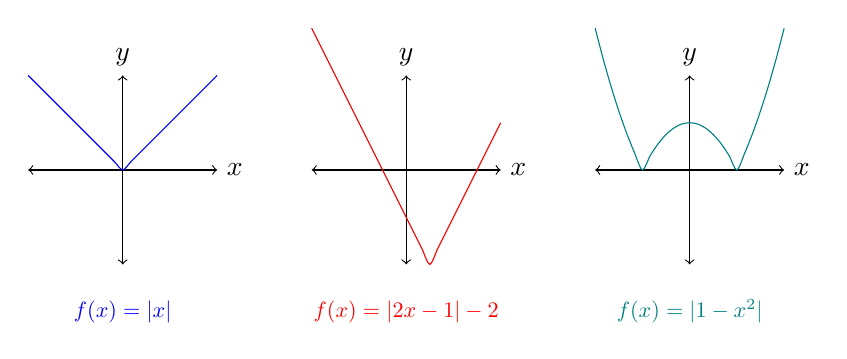
\begin{tikzpicture}[scale = 0.6, smooth, domain = -2:2]
\axes{-2}{2}{-2}{2};
\draw[blue] plot[domain = -2:2] (\x, {abs(\x)});
\node[blue, scale = 0.8] at (0,-3) {$f(x) = |x|$};
\begin{scope}[xshift = 6cm]
\axes{-2}{2}{-2}{2};
\draw[red] plot[domain = -2:2] (\x, {abs(2*\x-1)-2});
\node[red, scale = 0.8] at (0,-3) {$f(x) = |2x-1|-2$};
\end{scope}
\begin{scope}[xshift = 12cm]
\axes{-2}{2}{-2}{2};
\draw[teal] plot[domain = -2:2] (\x, {abs(1-\x*\x)});
\node[teal, scale = 0.8] at (0,-3) {$f(x) = |1-x^2|$};
\end{scope}
\end{tikzpicture}
\caption{Absolute value functions}
\end{figure}
\end{frame}

\begin{frame}
\frametitle{Step function}
7.  Step function - defined differently on intervals, so it looks like a staircase.

\begin{figure}[h!]
\centering
\begin{tikzpicture}[scale = 0.6]
\axes{-2}{2}{-2}{2};
\draw[blue] (-2,-1) -- (0,-1) (0,1) -- (2,1) (0,-1) circle [radius = 0.1cm];
\filldraw (0,1) circle [radius = 0.1cm];
\node[blue, scale = 0.8] at (0,-3) {$f(x) = \begin{cases} -1; & x < 0 \\ 1;&x \geq 0\end{cases}$};
\begin{scope}[xshift = 6cm]
\axes{-2}{2}{-2}{2};
\draw[red] (-2,2) -- (-1,2) (-1,-1) -- (1,-1) (1,0) -- (2,0) (-1,2) circle [radius = 0.1cm] (1,0) circle [radius = 0.1cm];
\filldraw (-1,-1) circle [radius = 0.1cm] (1,-1) circle [radius = 0.1cm];
\node[red, scale = 0.8] at (0,-3) {$f(x) = \begin{cases} 2; & x < -1 \\ -1;&-1 \leq x \leq 1 \\ 0; & x > 1\end{cases}$};
\end{scope}
\begin{scope}[xshift = 12cm]
\axes{-2}{2}{-2}{2};
\foreach \x in {-2,-1,0,1}
{
	\draw[teal] (\x, \x) -- ({\x+1}, \x) circle [radius = 0.1cm];
	\filldraw[teal] (\x, \x) circle [radius = 0.1cm];
}
\node[teal, scale = 0.8] at (0,-3) {$f(x) = \lfloor x \rfloor$};
\end{scope}
\end{tikzpicture}
\caption{Step functions}
\end{figure}
\end{frame}

\begin{frame}
\begin{exercisebox}{}
Graph the following functions for $x$ in $[0,2]$.
\begin{enumerate}
\item $f(x) = \lfloor x \rfloor$ where $\lfloor x \rfloor$ is the largest integer that is smaller than or equals to $x$. 

For instance $f(1.1) = 1, f(2.9) = 2, f(-1.5)=-2, f(5)=5$
\item $f(x) =$ the fractional part of $x$. 

For instance, $f(1.2) = 0.2, f(-2.01) = 0.01, f(4) = 0$
\end{enumerate}
\end{exercisebox}
\end{frame}

%%%%%%%%%%%%%%
\section{Using Graph}
\frame{\sectionpage}
%%%%%%%%%%%%%%

\begin{frame}
\frametitle{Graph Intersection}
You can use graph to \textbf{find} solutions to some problems. Suppose that we have graphs for $y = f(x)$ and $y = g(x)$. Let $(a,b)$ be an intersection of the graphs. Then we know that
\[ b = f(a) \text{ and } b = g(a) \]
Thus, we have $f(a) = g(a)$. This implies that $x=a$ is the solution to
\begin{block}{}
\[f(x) = g(x)\]
\end{block}
This works if the solutions are simple decimals, or if you only want an approximation. You still need to solve the equation algebraically if you want an exact answer that is irrational, like $x = \sqrt{3}-1$.
\end{frame}



\begin{frame}[t]
\begin{ex}
Use graphs to find the solutions of
\[ x+1 = 2x-4\]
\end{ex}
\begin{sol}
We plot the graphs of the function $f(x) = x+1$ and $g(x) = 2x-4$ and see that the intersection is at the point $(5,6)$. Thus, the solution is $x = 5$.
\addfig{0.6}{graph_intersection_ex1}{The intersection of $f(x) = x+1$ and $g(x) = 2x-4$.}{}
\end{sol}
\end{frame}


\begin{frame}[t]
\begin{ex}
Use graphs to find the solutions of
\[ x^2 = x\]
\end{ex}

\begin{sol}
We plot the graphs of the function $f(x) = x^2$ and $g(x) = x$ and see that the intersections are at the points $(0,0)$ and $(1,1)$. Thus, the solutions are $x = 0$ and $x=1$.
\addfig{0.5}{graph_intersection_ex2}{The intersections of $f(x) = x^2$ and $g(x) = x$.}{}
\end{sol}
\end{frame}

\begin{frame}
\frametitle{Graph Comparison}
Similarly, we can compare the graph of $y = f(x)$ and $y = g(x)$ to solve an inequality of the form
\[ f(x) \geq g(x)\]
The solutions will be intervals with intersections as the left end or the right end of the intervals.
\end{frame}


\begin{frame}[t]
\begin{ex}
Use graphs to find the solutions of
\[ x \geq x^2\]
\end{ex}
\begin{sol}
We plot the graphs of the function $f(x) = x$ and $g(x) = x^2$ and see that the part where $f(x) \geq g(x)$ is when $0 \leq x \leq 1$. Thus, the solutions are in the closed interval $[0, 1]$.
\addfig{0.5}{graph_ineq_ex1}{The region where of $f(x) \geq g(x)$.}{}
\end{sol}
\end{frame}


\begin{frame}[t]
\begin{ex}
Use graphs to find the solutions of
\[ x^2-3x+3 \geq 1\]
\end{ex}
\begin{sol}
We plot the graphs of the function $f(x) = x^2-3x+3$ and $g(x) = 1$ (which is a constant function) and see that the region where $f(x) \geq g(x)$ is when $x \leq 1$ or $x \geq 2$. Thus, the solutions are in the union of intervals $(-\infty, 1) \cup (2, \infty)$.
\addfig{0.5}{graph_ineq_ex2}{The region where of $f(x) \geq g(x)$.}{}
\end{sol}
\end{frame}

\begin{frame}
\begin{exercisebox}{}
Use desmos.com (or your favorite graphing tool) to find the solutions of the following equations or inequalities.
\begin{enumerate}
\item $3x+1 = 2x+4$
\item $x^2 = x+2$
\item $x^2-3x+2=0$
\item $x = \frac{1}{x}$
\item $x^2-3x+2 \leq 0$
\end{enumerate}
\end{exercisebox}
\end{frame}

%%%%%%%%%%%%%%
\section{Activity}
\frame{\sectionpage}
%%%%%%%%%%%%%%

\iffalse
\begin{frame}
\begin{exercisebox}{}
1. Google for your favorite/cool looking/bizarre/cute/funny graph.
\begin{figure}[h!]
\centering

\includegraphics[width = 0.7\textwidth]{l07i20.png}
\caption{\href{desmos.com/calculator}{Desmos.com}}
\end{figure}
\end{exercisebox}
\end{frame}
\fi

\begin{frame}
\begin{exercisebox}{}
Save the Princess and screencap it! You only need to submit the last one, but it's recommended you finish World 1-1 and 1-2 to understand the mechanism.
\begin{figure}[h!]
\centering

\includegraphics[width = 0.7\textwidth]{l07i21.png}
\caption{\href{https://teacher.desmos.com/activitybuilder/custom/5c7614041509d870d4838bfd}{Super Mario Quadratics}}
\end{figure}
\end{exercisebox}
\end{frame}

%%%%%%%%%%%%%%
\section{Extra}
\frame{\sectionpage}
%%%%%%%%%%%%%%

\begin{frame}
\frametitle{Graph as Recreation}
\begin{figure}[h!]
\centering

\includegraphics[width = 0.9\textwidth]{l07i17.png}
\caption{\href{https://www.youtube.com/watch?v=pAMgUB51XZA}{Amazing Graphs - Numberphile}}
\end{figure}
\end{frame}


\begin{frame}
\frametitle{Polar Coordinate}
\addfig{0.5}{graph_polar}{Polar Coordinate}{}
\end{frame}

